\documentclass[1p]{elsarticle_modified}
%\bibliographystyle{elsarticle-num}

%\usepackage[colorlinks]{hyperref}
%\usepackage{abbrmath_seonhwa} %\Abb, \Ascr, \Acal ,\Abf, \Afrak
\usepackage{amsfonts}
\usepackage{amssymb}
\usepackage{amsmath}
\usepackage{amsthm}
\usepackage{scalefnt}
\usepackage{amsbsy}
\usepackage{kotex}
\usepackage{caption}
\usepackage{subfig}
\usepackage{color}
\usepackage{graphicx}
\usepackage{xcolor} %% white, black, red, green, blue, cyan, magenta, yellow
\usepackage{float}
\usepackage{setspace}
\usepackage{hyperref}

\usepackage{tikz}
\usetikzlibrary{arrows}

\usepackage{multirow}
\usepackage{array} % fixed length table
\usepackage{hhline}

%%%%%%%%%%%%%%%%%%%%%
\makeatletter
\renewcommand*\env@matrix[1][\arraystretch]{%
	\edef\arraystretch{#1}%
	\hskip -\arraycolsep
	\let\@ifnextchar\new@ifnextchar
	\array{*\c@MaxMatrixCols c}}
\makeatother %https://tex.stackexchange.com/questions/14071/how-can-i-increase-the-line-spacing-in-a-matrix
%%%%%%%%%%%%%%%

\usepackage[normalem]{ulem}

\newcommand{\msout}[1]{\ifmmode\text{\sout{\ensuremath{#1}}}\else\sout{#1}\fi}
%SOURCE: \msout is \stkout macro in https://tex.stackexchange.com/questions/20609/strikeout-in-math-mode

\newcommand{\cancel}[1]{
	\ifmmode
	{\color{red}\msout{#1}}
	\else
	{\color{red}\sout{#1}}
	\fi
}

\newcommand{\add}[1]{
	{\color{blue}\uwave{#1}}
}

\newcommand{\replace}[2]{
	\ifmmode
	{\color{red}\msout{#1}}{\color{blue}\uwave{#2}}
	\else
	{\color{red}\sout{#1}}{\color{blue}\uwave{#2}}
	\fi
}

\newcommand{\Sol}{\mathcal{S}} %segment
\newcommand{\D}{D} %diagram
\newcommand{\A}{\mathcal{A}} %arc


%%%%%%%%%%%%%%%%%%%%%%%%%%%%%5 test

\def\sl{\operatorname{\textup{SL}}(2,\Cbb)}
\def\psl{\operatorname{\textup{PSL}}(2,\Cbb)}
\def\quan{\mkern 1mu \triangleright \mkern 1mu}

\theoremstyle{definition}
\newtheorem{thm}{Theorem}[section]
\newtheorem{prop}[thm]{Proposition}
\newtheorem{lem}[thm]{Lemma}
\newtheorem{ques}[thm]{Question}
\newtheorem{cor}[thm]{Corollary}
\newtheorem{defn}[thm]{Definition}
\newtheorem{exam}[thm]{Example}
\newtheorem{rmk}[thm]{Remark}
\newtheorem{alg}[thm]{Algorithm}

\newcommand{\I}{\sqrt{-1}}
\begin{document}

%\begin{frontmatter}
%
%\title{Boundary parabolic representations of knots up to 8 crossings}
%
%%% Group authors per affiliation:
%\author{Yunhi Cho} 
%\address{Department of Mathematics, University of Seoul, Seoul, Korea}
%\ead{yhcho@uos.ac.kr}
%
%
%\author{Seonhwa Kim} %\fnref{s_kim}}
%\address{Center for Geometry and Physics, Institute for Basic Science, Pohang, 37673, Korea}
%\ead{ryeona17@ibs.re.kr}
%
%\author{Hyuk Kim}
%\address{Department of Mathematical Sciences, Seoul National University, Seoul 08826, Korea}
%\ead{hyukkim@snu.ac.kr}
%
%\author{Seokbeom Yoon}
%\address{Department of Mathematical Sciences, Seoul National University, Seoul, 08826,  Korea}
%\ead{sbyoon15@snu.ac.kr}
%
%\begin{abstract}
%We find all boundary parabolic representation of knots up to 8 crossings.
%
%\end{abstract}
%\begin{keyword}
%    \MSC[2010] 57M25 
%\end{keyword}
%
%\end{frontmatter}

%\linenumbers
%\tableofcontents
%
\newcommand\colored[1]{\textcolor{white}{\rule[-0.35ex]{0.8em}{1.4ex}}\kern-0.8em\color{red} #1}%
%\newcommand\colored[1]{\textcolor{white}{ #1}\kern-2.17ex	\textcolor{white}{ #1}\kern-1.81ex	\textcolor{white}{ #1}\kern-2.15ex\color{red}#1	}

{\Large $\underline{11n_{25}~(K11n_{25})}$}

\setlength{\tabcolsep}{10pt}
\renewcommand{\arraystretch}{1.6}
\vspace{1cm}\begin{tabular}{m{100pt}>{\centering\arraybackslash}m{274pt}}
\multirow{5}{120pt}{
	\centering
	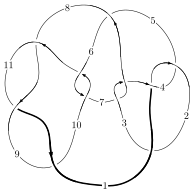
\includegraphics[width=112pt]{../../../GIT/diagram.site/Diagrams/png/641_11n_25.png}\\
\ \ \ A knot diagram\footnotemark}&
\allowdisplaybreaks
\textbf{Linearized knot diagam} \\
\cline{2-2}
 &
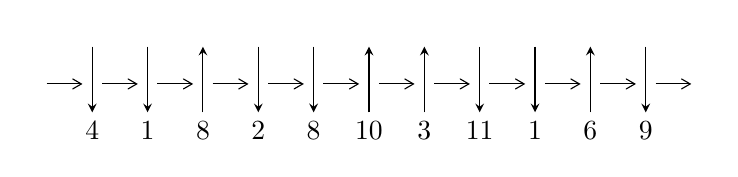
\begin{tikzpicture}[x=20pt, y=17pt]
	% nodes
	\node (C0) at (0, 0) {};
	\node (C1) at (1, 0) {};
	\node (C1U) at (1, +1) {};
	\node (C1D) at (1, -1) {4};

	\node (C2) at (2, 0) {};
	\node (C2U) at (2, +1) {};
	\node (C2D) at (2, -1) {1};

	\node (C3) at (3, 0) {};
	\node (C3U) at (3, +1) {};
	\node (C3D) at (3, -1) {8};

	\node (C4) at (4, 0) {};
	\node (C4U) at (4, +1) {};
	\node (C4D) at (4, -1) {2};

	\node (C5) at (5, 0) {};
	\node (C5U) at (5, +1) {};
	\node (C5D) at (5, -1) {8};

	\node (C6) at (6, 0) {};
	\node (C6U) at (6, +1) {};
	\node (C6D) at (6, -1) {10};

	\node (C7) at (7, 0) {};
	\node (C7U) at (7, +1) {};
	\node (C7D) at (7, -1) {3};

	\node (C8) at (8, 0) {};
	\node (C8U) at (8, +1) {};
	\node (C8D) at (8, -1) {11};

	\node (C9) at (9, 0) {};
	\node (C9U) at (9, +1) {};
	\node (C9D) at (9, -1) {1};

	\node (C10) at (10, 0) {};
	\node (C10U) at (10, +1) {};
	\node (C10D) at (10, -1) {6};

	\node (C11) at (11, 0) {};
	\node (C11U) at (11, +1) {};
	\node (C11D) at (11, -1) {9};
	\node (C12) at (12, 0) {};

	% arrows
	\draw[->,>={angle 60}]
	(C0) edge (C1) (C1) edge (C2) (C2) edge (C3) (C3) edge (C4) (C4) edge (C5) (C5) edge (C6) (C6) edge (C7) (C7) edge (C8) (C8) edge (C9) (C9) edge (C10) (C10) edge (C11) (C11) edge (C12) ;	\draw[->,>=stealth]
	(C1U) edge (C1D) (C2U) edge (C2D) (C3D) edge (C3U) (C4U) edge (C4D) (C5U) edge (C5D) (C6D) edge (C6U) (C7D) edge (C7U) (C8U) edge (C8D) (C9U) edge (C9D) (C10D) edge (C10U) (C11U) edge (C11D) ;
	\end{tikzpicture} \\
\hhline{~~} \\& 
\textbf{Solving Sequence} \\ \cline{2-2} 
 &
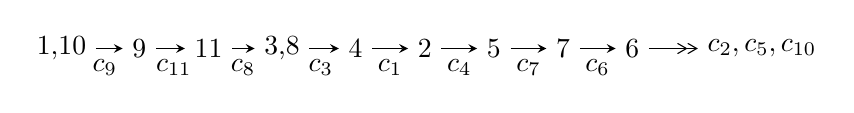
\begin{tikzpicture}[x=25pt, y=7pt]
	% node
	\node (A0) at (-1/8, 0) {1,10};
	\node (A1) at (1, 0) {9};
	\node (A2) at (2, 0) {11};
	\node (A3) at (49/16, 0) {3,8};
	\node (A4) at (33/8, 0) {4};
	\node (A5) at (41/8, 0) {2};
	\node (A6) at (49/8, 0) {5};
	\node (A7) at (57/8, 0) {7};
	\node (A8) at (65/8, 0) {6};
	\node (C1) at (1/2, -1) {$c_{9}$};
	\node (C2) at (3/2, -1) {$c_{11}$};
	\node (C3) at (5/2, -1) {$c_{8}$};
	\node (C4) at (29/8, -1) {$c_{3}$};
	\node (C5) at (37/8, -1) {$c_{1}$};
	\node (C6) at (45/8, -1) {$c_{4}$};
	\node (C7) at (53/8, -1) {$c_{7}$};
	\node (C8) at (61/8, -1) {$c_{6}$};
	\node (A9) at (10, 0) {$c_{2},c_{5},c_{10}$};

	% edge
	\draw[->,>=stealth]	
	(A0) edge (A1) (A1) edge (A2) (A2) edge (A3) (A3) edge (A4) (A4) edge (A5) (A5) edge (A6) (A6) edge (A7) (A7) edge (A8) ;
	\draw[->>,>={angle 60}]	
	(A8) edge (A9);
\end{tikzpicture} \\ 

\end{tabular} \\

\footnotetext{
The image of knot diagram is generated by the software ``\textbf{Draw programme}" developed by Andrew Bartholomew(\url{http://www.layer8.co.uk/maths/draw/index.htm\#Running-draw}), where we modified some parts for our purpose(\url{https://github.com/CATsTAILs/LinksPainter}).
}\phantom \\ \newline 
\centering \textbf{Ideals for irreducible components\footnotemark of $X_{\text{par}}$} 
 
\begin{align*}
I^u_{1}&=\langle 
-78512077 u^{27}-145372804 u^{26}+\cdots+67221149 b-176175,\\
\phantom{I^u_{1}}&\phantom{= \langle  }-62468877 u^{27}-129722654 u^{26}+\cdots+67221149 a+343854265,\;u^{28}+2 u^{27}+\cdots-5 u+1\rangle \\
I^u_{2}&=\langle 
u^4+u^3- u^2+b- u,\;u^4+u^3-2 u^2+a- u+1,\;u^5+u^4-2 u^3- u^2+u-1\rangle \\
\\
\end{align*}
\raggedright * 2 irreducible components of $\dim_{\mathbb{C}}=0$, with total 33 representations.\\
\footnotetext{All coefficients of polynomials are rational numbers. But the coefficients are sometimes approximated in decimal forms when there is not enough margin.}
\newpage
\renewcommand{\arraystretch}{1}
\centering \section*{I. $I^u_{1}= \langle -7.85\times10^{7} u^{27}-1.45\times10^{8} u^{26}+\cdots+6.72\times10^{7} b-1.76\times10^{5},\;-6.25\times10^{7} u^{27}-1.30\times10^{8} u^{26}+\cdots+6.72\times10^{7} a+3.44\times10^{8},\;u^{28}+2 u^{27}+\cdots-5 u+1 \rangle$}
\flushleft \textbf{(i) Arc colorings}\\
\begin{tabular}{m{7pt} m{180pt} m{7pt} m{180pt} }
\flushright $a_{1}=$&$\begin{pmatrix}0\\u\end{pmatrix}$ \\
\flushright $a_{10}=$&$\begin{pmatrix}1\\0\end{pmatrix}$ \\
\flushright $a_{9}=$&$\begin{pmatrix}1\\- u^2\end{pmatrix}$ \\
\flushright $a_{11}=$&$\begin{pmatrix}u\\- u^3+u\end{pmatrix}$ \\
\flushright $a_{3}=$&$\begin{pmatrix}0.929304 u^{27}+1.92979 u^{26}+\cdots+11.1441 u-5.11527\\1.16797 u^{27}+2.16261 u^{26}+\cdots+2.86935 u+0.00262083\end{pmatrix}$ \\
\flushright $a_{8}=$&$\begin{pmatrix}- u^2+1\\u^4-2 u^2\end{pmatrix}$ \\
\flushright $a_{4}=$&$\begin{pmatrix}1.01767 u^{27}+2.01755 u^{26}+\cdots+12.4640 u-4.97118\\0.885451 u^{27}+1.93727 u^{26}+\cdots+3.16598 u-0.0228994\end{pmatrix}$ \\
\flushright $a_{2}=$&$\begin{pmatrix}0.929304 u^{27}+1.92979 u^{26}+\cdots+11.1441 u-5.11527\\1.40015 u^{27}+2.23327 u^{26}+\cdots+3.44274 u+0.0738023\end{pmatrix}$ \\
\flushright $a_{5}=$&$\begin{pmatrix}0.823260 u^{27}+0.824473 u^{26}+\cdots+0.360292 u+0.711827\\-2.02865 u^{27}-1.42566 u^{26}+\cdots+4.66019 u-0.824392\end{pmatrix}$ \\
\flushright $a_{7}=$&$\begin{pmatrix}-1.43559 u^{27}-1.43578 u^{26}+\cdots+3.66414 u-1.71740\\1.00626 u^{27}+1.00303 u^{26}+\cdots-0.736587 u+0.00303364\end{pmatrix}$ \\
\flushright $a_{6}=$&$\begin{pmatrix}-2.44185 u^{27}-2.43882 u^{26}+\cdots+4.40073 u-1.72043\\1.00626 u^{27}+1.00303 u^{26}+\cdots-0.736587 u+0.00303364\end{pmatrix}$\\ \flushright $a_{6}=$&$\begin{pmatrix}-2.44185 u^{27}-2.43882 u^{26}+\cdots+4.40073 u-1.72043\\1.00626 u^{27}+1.00303 u^{26}+\cdots-0.736587 u+0.00303364\end{pmatrix}$\\&\end{tabular}
\flushleft \textbf{(ii) Obstruction class $= -1$}\\~\\
\flushleft \textbf{(iii) Cusp Shapes $= -\frac{337541215}{67221149} u^{27}-\frac{737621299}{67221149} u^{26}+\cdots-\frac{124989334}{67221149} u-\frac{310642967}{67221149}$}\\~\\
\newpage\renewcommand{\arraystretch}{1}
\flushleft \textbf{(iv) u-Polynomials at the component}\newline \\
\begin{tabular}{m{50pt}|m{274pt}}
Crossings & \hspace{64pt}u-Polynomials at each crossing \\
\hline $$\begin{aligned}c_{1},c_{4}\end{aligned}$$&$\begin{aligned}
&u^{28}-6 u^{27}+\cdots+5 u-1
\end{aligned}$\\
\hline $$\begin{aligned}c_{2}\end{aligned}$$&$\begin{aligned}
&u^{28}+6 u^{27}+\cdots+17 u+1
\end{aligned}$\\
\hline $$\begin{aligned}c_{3},c_{7}\end{aligned}$$&$\begin{aligned}
&u^{28}+3 u^{27}+\cdots+128 u+32
\end{aligned}$\\
\hline $$\begin{aligned}c_{5}\end{aligned}$$&$\begin{aligned}
&u^{28}-6 u^{27}+\cdots-3079 u-1609
\end{aligned}$\\
\hline $$\begin{aligned}c_{6},c_{10}\end{aligned}$$&$\begin{aligned}
&u^{28}-2 u^{27}+\cdots+u-1
\end{aligned}$\\
\hline $$\begin{aligned}c_{8},c_{9},c_{11}\end{aligned}$$&$\begin{aligned}
&u^{28}-2 u^{27}+\cdots+5 u+1
\end{aligned}$\\
\hline
\end{tabular}\\~\\
\newpage\renewcommand{\arraystretch}{1}
\flushleft \textbf{(v) Riley Polynomials at the component}\newline \\
\begin{tabular}{m{50pt}|m{274pt}}
Crossings & \hspace{64pt}Riley Polynomials at each crossing \\
\hline $$\begin{aligned}c_{1},c_{4}\end{aligned}$$&$\begin{aligned}
&y^{28}-6 y^{27}+\cdots-17 y+1
\end{aligned}$\\
\hline $$\begin{aligned}c_{2}\end{aligned}$$&$\begin{aligned}
&y^{28}+38 y^{27}+\cdots-17 y+1
\end{aligned}$\\
\hline $$\begin{aligned}c_{3},c_{7}\end{aligned}$$&$\begin{aligned}
&y^{28}-33 y^{27}+\cdots-14848 y+1024
\end{aligned}$\\
\hline $$\begin{aligned}c_{5}\end{aligned}$$&$\begin{aligned}
&y^{28}+22 y^{27}+\cdots+19658749 y+2588881
\end{aligned}$\\
\hline $$\begin{aligned}c_{6},c_{10}\end{aligned}$$&$\begin{aligned}
&y^{28}+6 y^{27}+\cdots+5 y+1
\end{aligned}$\\
\hline $$\begin{aligned}c_{8},c_{9},c_{11}\end{aligned}$$&$\begin{aligned}
&y^{28}-22 y^{27}+\cdots+5 y+1
\end{aligned}$\\
\hline
\end{tabular}\\~\\
\newpage\flushleft \textbf{(vi) Complex Volumes and Cusp Shapes}
$$\begin{array}{c|c|c}  
\text{Solutions to }I^u_{1}& \I (\text{vol} + \sqrt{-1}CS) & \text{Cusp shape}\\
 \hline 
\begin{aligned}
u &= \phantom{-}0.078918 + 0.962099 I \\
a &= -2.18951 + 0.08530 I \\
b &= -2.13157 + 0.38039 I\end{aligned}
 & \phantom{-}7.91461 - 7.14026 I & -1.25171 + 4.70902 I \\ \hline\begin{aligned}
u &= \phantom{-}0.078918 - 0.962099 I \\
a &= -2.18951 - 0.08530 I \\
b &= -2.13157 - 0.38039 I\end{aligned}
 & \phantom{-}7.91461 + 7.14026 I & -1.25171 - 4.70902 I \\ \hline\begin{aligned}
u &= \phantom{-}1.062800 + 0.195424 I \\
a &= -0.155091 - 0.173758 I \\
b &= \phantom{-}0.944249 + 0.890794 I\end{aligned}
 & -2.13241 - 0.82619 I & -5.35184 - 1.04773 I \\ \hline\begin{aligned}
u &= \phantom{-}1.062800 - 0.195424 I \\
a &= -0.155091 + 0.173758 I \\
b &= \phantom{-}0.944249 - 0.890794 I\end{aligned}
 & -2.13241 + 0.82619 I & -5.35184 + 1.04773 I \\ \hline\begin{aligned}
u &= -0.064858 + 0.917024 I \\
a &= \phantom{-}2.10546 - 0.51061 I \\
b &= \phantom{-}1.81015 - 0.32496 I\end{aligned}
 & \phantom{-}8.51104 + 0.29713 I & -0.154356 - 0.088934 I \\ \hline\begin{aligned}
u &= -0.064858 - 0.917024 I \\
a &= \phantom{-}2.10546 + 0.51061 I \\
b &= \phantom{-}1.81015 + 0.32496 I\end{aligned}
 & \phantom{-}8.51104 - 0.29713 I & -0.154356 + 0.088934 I \\ \hline\begin{aligned}
u &= \phantom{-}1.08514\phantom{ +0.000000I} \\
a &= -1.05851\phantom{ +0.000000I} \\
b &= -3.52629\phantom{ +0.000000I}\end{aligned}
 & -3.64067\phantom{ +0.000000I} & \phantom{-}25.0750\phantom{ +0.000000I} \\ \hline\begin{aligned}
u &= -1.206550 + 0.074740 I \\
a &= \phantom{-}1.56629 - 0.83850 I \\
b &= \phantom{-}0.209734 + 0.919216 I\end{aligned}
 & -5.80044 + 1.71298 I & -12.51650 - 3.41779 I \\ \hline\begin{aligned}
u &= -1.206550 - 0.074740 I \\
a &= \phantom{-}1.56629 + 0.83850 I \\
b &= \phantom{-}0.209734 - 0.919216 I\end{aligned}
 & -5.80044 - 1.71298 I & -12.51650 + 3.41779 I \\ \hline\begin{aligned}
u &= -1.184170 + 0.243247 I \\
a &= -0.333050 - 1.009550 I \\
b &= \phantom{-}0.117217 + 0.500518 I\end{aligned}
 & -2.65368 + 4.42550 I & -6.50791 - 7.50568 I\\
 \hline 
 \end{array}$$\newpage$$\begin{array}{c|c|c}  
\text{Solutions to }I^u_{1}& \I (\text{vol} + \sqrt{-1}CS) & \text{Cusp shape}\\
 \hline 
\begin{aligned}
u &= -1.184170 - 0.243247 I \\
a &= -0.333050 + 1.009550 I \\
b &= \phantom{-}0.117217 - 0.500518 I\end{aligned}
 & -2.65368 - 4.42550 I & -6.50791 + 7.50568 I \\ \hline\begin{aligned}
u &= \phantom{-}0.429683 + 0.631440 I \\
a &= -0.286291 - 0.034580 I \\
b &= \phantom{-}0.231084 + 0.498413 I\end{aligned}
 & -0.69638 - 1.96456 I & -1.12748 + 4.70329 I \\ \hline\begin{aligned}
u &= \phantom{-}0.429683 - 0.631440 I \\
a &= -0.286291 + 0.034580 I \\
b &= \phantom{-}0.231084 - 0.498413 I\end{aligned}
 & -0.69638 + 1.96456 I & -1.12748 - 4.70329 I \\ \hline\begin{aligned}
u &= \phantom{-}1.29906\phantom{ +0.000000I} \\
a &= -0.104420\phantom{ +0.000000I} \\
b &= \phantom{-}0.740536\phantom{ +0.000000I}\end{aligned}
 & -2.76755\phantom{ +0.000000I} & -1.63490\phantom{ +0.000000I} \\ \hline\begin{aligned}
u &= -1.238710 + 0.461764 I \\
a &= -1.08774 + 1.05934 I \\
b &= -1.71542 - 0.63051 I\end{aligned}
 & \phantom{-}4.88950 + 4.61956 I & -3.15122 - 3.64430 I \\ \hline\begin{aligned}
u &= -1.238710 - 0.461764 I \\
a &= -1.08774 - 1.05934 I \\
b &= -1.71542 + 0.63051 I\end{aligned}
 & \phantom{-}4.88950 - 4.61956 I & -3.15122 + 3.64430 I \\ \hline\begin{aligned}
u &= \phantom{-}1.236490 + 0.512229 I \\
a &= \phantom{-}0.561715 + 1.232250 I \\
b &= \phantom{-}2.01617 - 0.03791 I\end{aligned}
 & \phantom{-}4.35345 + 1.91548 I & -3.75065 - 1.71492 I \\ \hline\begin{aligned}
u &= \phantom{-}1.236490 - 0.512229 I \\
a &= \phantom{-}0.561715 - 1.232250 I \\
b &= \phantom{-}2.01617 + 0.03791 I\end{aligned}
 & \phantom{-}4.35345 - 1.91548 I & -3.75065 + 1.71492 I \\ \hline\begin{aligned}
u &= \phantom{-}1.338030 + 0.423130 I \\
a &= -0.503580 - 1.252560 I \\
b &= -1.76982 - 0.03806 I\end{aligned}
 & \phantom{-}4.11604 - 5.09421 I & -3.90084 + 3.07789 I \\ \hline\begin{aligned}
u &= \phantom{-}1.338030 - 0.423130 I \\
a &= -0.503580 + 1.252560 I \\
b &= -1.76982 + 0.03806 I\end{aligned}
 & \phantom{-}4.11604 + 5.09421 I & -3.90084 - 3.07789 I\\
 \hline 
 \end{array}$$\newpage$$\begin{array}{c|c|c}  
\text{Solutions to }I^u_{1}& \I (\text{vol} + \sqrt{-1}CS) & \text{Cusp shape}\\
 \hline 
\begin{aligned}
u &= -1.35468 + 0.45041 I \\
a &= \phantom{-}0.88989 - 1.31460 I \\
b &= \phantom{-}2.05008 + 0.73045 I\end{aligned}
 & \phantom{-}3.42542 + 12.18300 I & -4.89577 - 7.01706 I \\ \hline\begin{aligned}
u &= -1.35468 - 0.45041 I \\
a &= \phantom{-}0.88989 + 1.31460 I \\
b &= \phantom{-}2.05008 - 0.73045 I\end{aligned}
 & \phantom{-}3.42542 - 12.18300 I & -4.89577 + 7.01706 I \\ \hline\begin{aligned}
u &= -0.018893 + 0.524896 I \\
a &= -0.530824 - 0.538417 I \\
b &= -0.574926 + 0.352337 I\end{aligned}
 & \phantom{-}0.76347 - 1.52310 I & \phantom{-}1.12747 + 4.03193 I \\ \hline\begin{aligned}
u &= -0.018893 - 0.524896 I \\
a &= -0.530824 + 0.538417 I \\
b &= -0.574926 - 0.352337 I\end{aligned}
 & \phantom{-}0.76347 + 1.52310 I & \phantom{-}1.12747 - 4.03193 I \\ \hline\begin{aligned}
u &= -1.46446 + 0.20354 I \\
a &= \phantom{-}0.333881 - 0.215100 I \\
b &= -0.390847 + 0.079026 I\end{aligned}
 & -6.89024 + 4.97150 I & -3.93501 - 6.51666 I \\ \hline\begin{aligned}
u &= -1.46446 - 0.20354 I \\
a &= \phantom{-}0.333881 + 0.215100 I \\
b &= -0.390847 - 0.079026 I\end{aligned}
 & -6.89024 - 4.97150 I & -3.93501 + 6.51666 I \\ \hline\begin{aligned}
u &= \phantom{-}0.194298 + 0.209673 I \\
a &= -3.28968 + 1.85114 I \\
b &= \phantom{-}0.596766 + 1.022050 I\end{aligned}
 & -1.90419 - 0.70187 I & -5.30439 - 2.49815 I \\ \hline\begin{aligned}
u &= \phantom{-}0.194298 - 0.209673 I \\
a &= -3.28968 - 1.85114 I \\
b &= \phantom{-}0.596766 - 1.022050 I\end{aligned}
 & -1.90419 + 0.70187 I & -5.30439 + 2.49815 I\\
 \hline 
 \end{array}$$\newpage\newpage\renewcommand{\arraystretch}{1}
\centering \section*{II. $I^u_{2}= \langle u^4+u^3- u^2+b- u,\;u^4+u^3-2 u^2+a- u+1,\;u^5+u^4-2 u^3- u^2+u-1 \rangle$}
\flushleft \textbf{(i) Arc colorings}\\
\begin{tabular}{m{7pt} m{180pt} m{7pt} m{180pt} }
\flushright $a_{1}=$&$\begin{pmatrix}0\\u\end{pmatrix}$ \\
\flushright $a_{10}=$&$\begin{pmatrix}1\\0\end{pmatrix}$ \\
\flushright $a_{9}=$&$\begin{pmatrix}1\\- u^2\end{pmatrix}$ \\
\flushright $a_{11}=$&$\begin{pmatrix}u\\- u^3+u\end{pmatrix}$ \\
\flushright $a_{3}=$&$\begin{pmatrix}- u^4- u^3+2 u^2+u-1\\- u^4- u^3+u^2+u\end{pmatrix}$ \\
\flushright $a_{8}=$&$\begin{pmatrix}- u^2+1\\u^4-2 u^2\end{pmatrix}$ \\
\flushright $a_{4}=$&$\begin{pmatrix}- u^4- u^3+2 u^2+u-1\\- u^4- u^3+u^2+u\end{pmatrix}$ \\
\flushright $a_{2}=$&$\begin{pmatrix}- u^4- u^3+2 u^2+u-1\\- u^4- u^3+u^2+2 u\end{pmatrix}$ \\
\flushright $a_{5}=$&$\begin{pmatrix}0\\- u\end{pmatrix}$ \\
\flushright $a_{7}=$&$\begin{pmatrix}- u^2+1\\u^4-2 u^2\end{pmatrix}$ \\
\flushright $a_{6}=$&$\begin{pmatrix}- u^4+u^2+1\\u^4-2 u^2\end{pmatrix}$\\ \flushright $a_{6}=$&$\begin{pmatrix}- u^4+u^2+1\\u^4-2 u^2\end{pmatrix}$\\&\end{tabular}
\flushleft \textbf{(ii) Obstruction class $= 1$}\\~\\
\flushleft \textbf{(iii) Cusp Shapes $= -2 u^4-5 u^3+2 u^2+8 u-10$}\\~\\
\newpage\renewcommand{\arraystretch}{1}
\flushleft \textbf{(iv) u-Polynomials at the component}\newline \\
\begin{tabular}{m{50pt}|m{274pt}}
Crossings & \hspace{64pt}u-Polynomials at each crossing \\
\hline $$\begin{aligned}c_{1}\end{aligned}$$&$\begin{aligned}
&(u-1)^5
\end{aligned}$\\
\hline $$\begin{aligned}c_{2},c_{4}\end{aligned}$$&$\begin{aligned}
&(u+1)^5
\end{aligned}$\\
\hline $$\begin{aligned}c_{3},c_{7}\end{aligned}$$&$\begin{aligned}
&u^5
\end{aligned}$\\
\hline $$\begin{aligned}c_{5}\end{aligned}$$&$\begin{aligned}
&u^5-3 u^4+4 u^3- u^2- u+1
\end{aligned}$\\
\hline $$\begin{aligned}c_{6}\end{aligned}$$&$\begin{aligned}
&u^5- u^4+2 u^3- u^2+u-1
\end{aligned}$\\
\hline $$\begin{aligned}c_{8},c_{9}\end{aligned}$$&$\begin{aligned}
&u^5+u^4-2 u^3- u^2+u-1
\end{aligned}$\\
\hline $$\begin{aligned}c_{10}\end{aligned}$$&$\begin{aligned}
&u^5+u^4+2 u^3+u^2+u+1
\end{aligned}$\\
\hline $$\begin{aligned}c_{11}\end{aligned}$$&$\begin{aligned}
&u^5- u^4-2 u^3+u^2+u+1
\end{aligned}$\\
\hline
\end{tabular}\\~\\
\newpage\renewcommand{\arraystretch}{1}
\flushleft \textbf{(v) Riley Polynomials at the component}\newline \\
\begin{tabular}{m{50pt}|m{274pt}}
Crossings & \hspace{64pt}Riley Polynomials at each crossing \\
\hline $$\begin{aligned}c_{1},c_{2},c_{4}\end{aligned}$$&$\begin{aligned}
&(y-1)^5
\end{aligned}$\\
\hline $$\begin{aligned}c_{3},c_{7}\end{aligned}$$&$\begin{aligned}
&y^5
\end{aligned}$\\
\hline $$\begin{aligned}c_{5}\end{aligned}$$&$\begin{aligned}
&y^5- y^4+8 y^3-3 y^2+3 y-1
\end{aligned}$\\
\hline $$\begin{aligned}c_{6},c_{10}\end{aligned}$$&$\begin{aligned}
&y^5+3 y^4+4 y^3+y^2- y-1
\end{aligned}$\\
\hline $$\begin{aligned}c_{8},c_{9},c_{11}\end{aligned}$$&$\begin{aligned}
&y^5-5 y^4+8 y^3-3 y^2- y-1
\end{aligned}$\\
\hline
\end{tabular}\\~\\
\newpage\flushleft \textbf{(vi) Complex Volumes and Cusp Shapes}
$$\begin{array}{c|c|c}  
\text{Solutions to }I^u_{2}& \I (\text{vol} + \sqrt{-1}CS) & \text{Cusp shape}\\
 \hline 
\begin{aligned}
u &= \phantom{-}1.21774\phantom{ +0.000000I} \\
a &= -0.821196\phantom{ +0.000000I} \\
b &= -1.30408\phantom{ +0.000000I}\end{aligned}
 & -4.04602\phantom{ +0.000000I} & -10.7190\phantom{ +0.000000I} \\ \hline\begin{aligned}
u &= \phantom{-}0.309916 + 0.549911 I \\
a &= -0.77780 + 1.38013 I \\
b &= \phantom{-}0.428550 + 1.039280 I\end{aligned}
 & -1.97403 - 1.53058 I & -6.52924 + 5.40154 I \\ \hline\begin{aligned}
u &= \phantom{-}0.309916 - 0.549911 I \\
a &= -0.77780 - 1.38013 I \\
b &= \phantom{-}0.428550 - 1.039280 I\end{aligned}
 & -1.97403 + 1.53058 I & -6.52924 - 5.40154 I \\ \hline\begin{aligned}
u &= -1.41878 + 0.21917 I \\
a &= \phantom{-}0.688402 + 0.106340 I \\
b &= -0.276511 + 0.728237 I\end{aligned}
 & -7.51750 + 4.40083 I & -11.11126 - 1.16747 I \\ \hline\begin{aligned}
u &= -1.41878 - 0.21917 I \\
a &= \phantom{-}0.688402 - 0.106340 I \\
b &= -0.276511 - 0.728237 I\end{aligned}
 & -7.51750 - 4.40083 I & -11.11126 + 1.16747 I\\
 \hline 
 \end{array}$$\newpage
\newpage\renewcommand{\arraystretch}{1}
\centering \section*{ III. u-Polynomials}
\begin{tabular}{m{50pt}|m{274pt}}
Crossings & \hspace{64pt}u-Polynomials at each crossing \\
\hline $$\begin{aligned}c_{1}\end{aligned}$$&$\begin{aligned}
&((u-1)^5)(u^{28}-6 u^{27}+\cdots+5 u-1)
\end{aligned}$\\
\hline $$\begin{aligned}c_{2}\end{aligned}$$&$\begin{aligned}
&((u+1)^5)(u^{28}+6 u^{27}+\cdots+17 u+1)
\end{aligned}$\\
\hline $$\begin{aligned}c_{3},c_{7}\end{aligned}$$&$\begin{aligned}
&u^5(u^{28}+3 u^{27}+\cdots+128 u+32)
\end{aligned}$\\
\hline $$\begin{aligned}c_{4}\end{aligned}$$&$\begin{aligned}
&((u+1)^5)(u^{28}-6 u^{27}+\cdots+5 u-1)
\end{aligned}$\\
\hline $$\begin{aligned}c_{5}\end{aligned}$$&$\begin{aligned}
&(u^5-3 u^4+4 u^3- u^2- u+1)(u^{28}-6 u^{27}+\cdots-3079 u-1609)
\end{aligned}$\\
\hline $$\begin{aligned}c_{6}\end{aligned}$$&$\begin{aligned}
&(u^5- u^4+2 u^3- u^2+u-1)(u^{28}-2 u^{27}+\cdots+u-1)
\end{aligned}$\\
\hline $$\begin{aligned}c_{8},c_{9}\end{aligned}$$&$\begin{aligned}
&(u^5+u^4-2 u^3- u^2+u-1)(u^{28}-2 u^{27}+\cdots+5 u+1)
\end{aligned}$\\
\hline $$\begin{aligned}c_{10}\end{aligned}$$&$\begin{aligned}
&(u^5+u^4+2 u^3+u^2+u+1)(u^{28}-2 u^{27}+\cdots+u-1)
\end{aligned}$\\
\hline $$\begin{aligned}c_{11}\end{aligned}$$&$\begin{aligned}
&(u^5- u^4-2 u^3+u^2+u+1)(u^{28}-2 u^{27}+\cdots+5 u+1)
\end{aligned}$\\
\hline
\end{tabular}\newpage\renewcommand{\arraystretch}{1}
\centering \section*{ IV. Riley Polynomials}
\begin{tabular}{m{50pt}|m{274pt}}
Crossings & \hspace{64pt}Riley Polynomials at each crossing \\
\hline $$\begin{aligned}c_{1},c_{4}\end{aligned}$$&$\begin{aligned}
&((y-1)^5)(y^{28}-6 y^{27}+\cdots-17 y+1)
\end{aligned}$\\
\hline $$\begin{aligned}c_{2}\end{aligned}$$&$\begin{aligned}
&((y-1)^5)(y^{28}+38 y^{27}+\cdots-17 y+1)
\end{aligned}$\\
\hline $$\begin{aligned}c_{3},c_{7}\end{aligned}$$&$\begin{aligned}
&y^5(y^{28}-33 y^{27}+\cdots-14848 y+1024)
\end{aligned}$\\
\hline $$\begin{aligned}c_{5}\end{aligned}$$&$\begin{aligned}
&(y^5- y^4+8 y^3-3 y^2+3 y-1)\\
&\cdot(y^{28}+22 y^{27}+\cdots+19658749 y+2588881)
\end{aligned}$\\
\hline $$\begin{aligned}c_{6},c_{10}\end{aligned}$$&$\begin{aligned}
&(y^5+3 y^4+4 y^3+y^2- y-1)(y^{28}+6 y^{27}+\cdots+5 y+1)
\end{aligned}$\\
\hline $$\begin{aligned}c_{8},c_{9},c_{11}\end{aligned}$$&$\begin{aligned}
&(y^5-5 y^4+8 y^3-3 y^2- y-1)(y^{28}-22 y^{27}+\cdots+5 y+1)
\end{aligned}$\\
\hline
\end{tabular}
\vskip 2pc
\end{document}